% SPDX-FileCopyrightText: 2026 Cyprien PIERRE
% SPDX-License-Identifier: CC-BY-4.0
\documentclass[tikz,border=5pt]{standalone}
\usepackage[T1]{fontenc}
\usepackage{lmodern}
\usetikzlibrary{arrows.meta,positioning}
\begin{document}
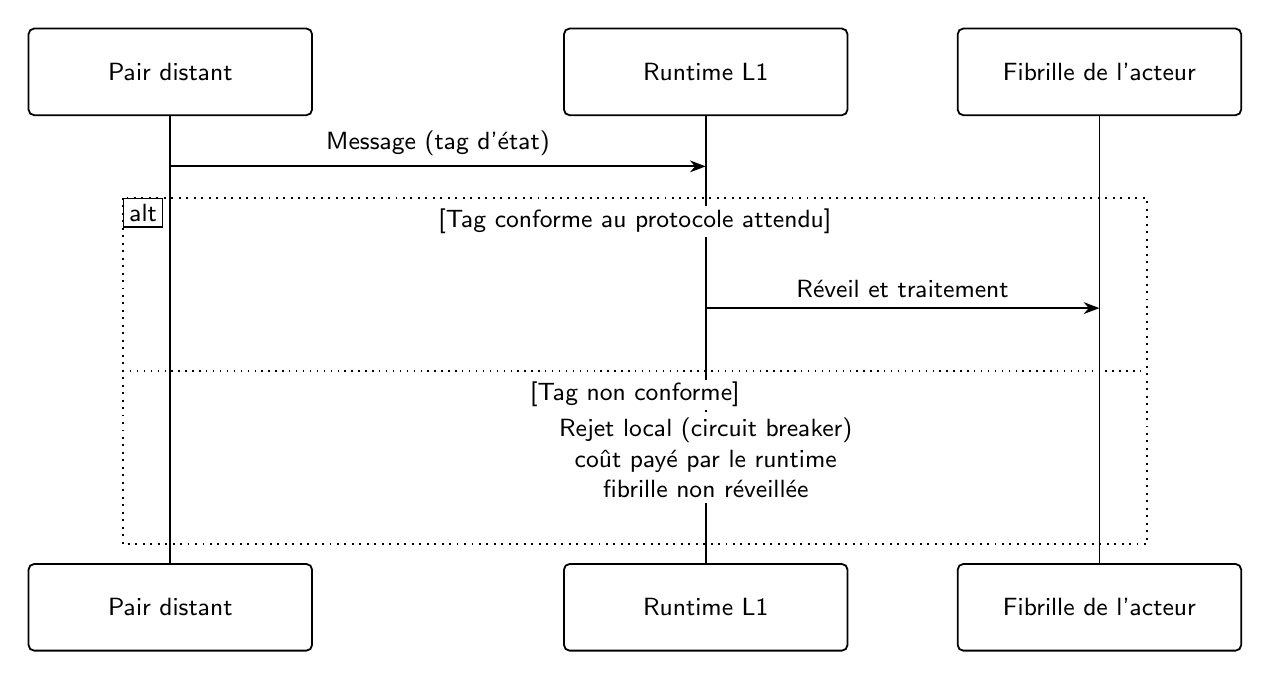
\begin{tikzpicture}[
  font=\sffamily\small,
  head/.style={draw, rounded corners=2pt, align=center, line width=.65pt, minimum height=11mm, minimum width=36mm},
  life/.style={line width=.65pt},
  message/.style={-{Stealth[length=2mm]}, line width=.7pt},
  fragment/.style={draw, dotted, line width=.7pt}
]
\node[head] (peer) at (0,0) {Pair distant};
\node[head] (rt) at (68mm,0) {Runtime L1};
\node[head] (fib) at (118mm,0) {Fibrille de l'acteur};
\node[head] (peer2) at (0,-68mm) {Pair distant};
\node[head] (rt2) at (68mm,-68mm) {Runtime L1};
\node[head] (fib2) at (118mm,-68mm) {Fibrille de l'acteur};
\draw[life] (peer) -- (peer2);
\draw[life] (rt) -- (rt2);
\draw[life] (fib) -- (fib2);
\draw[message] (0,-12mm) -- node[above] {Message (tag d'état)} (68mm,-12mm);
\draw[fragment] (-6mm,-16mm) rectangle (124mm,-60mm);
\node[draw, line width=.5pt, anchor=north west, inner sep=2pt] at (-6mm,-16mm) {alt};
\node[anchor=north, fill=white, inner sep=1pt] at (59mm,-17mm) {[Tag conforme au protocole attendu]};
\draw[message] (68mm,-30mm) -- node[above] {Réveil et traitement} (118mm,-30mm);
\draw[dotted, line width=.5pt] (-6mm,-38mm) -- (124mm,-38mm);
\node[anchor=north, fill=white, inner sep=1pt] at (59mm,-39mm) {[Tag non conforme]};
\node[align=center, fill=white, inner sep=2pt, text width=68mm] at (68mm,-49mm) {Rejet local (circuit breaker)\\coût payé par le runtime\\fibrille non réveillée};
\end{tikzpicture}
\end{document}
